\section{Processi di supporto}
	\subsection{Gestione della qualità}
		\subsubsection{Introduzione Processo}
			\paragraph{Descrizione}
				La garanzia della qualità si compone di diversi controlli che devono essere effettuati per:
				\begin{itemize}
					\item il software;
					\item la documentazione;
					\item tutti i processi che portano alla realizzazione della documentazione e del software.
				\end{itemize}
				Per ogni processo mirato alla qualità si definiscono delle metriche che vengono riportate in ciascuna sezione del presente documento. Nello specifico la descrizione di una norma in questo documento si compone dei seguenti attributi:
				\begin{itemize}
					\item\textbf{Descrizione}: descrive il valore e l’utilizzo della metrica
					\item\textbf{Unità di misura}: unità di misura della metrica;
					\item\textbf{Fonte}: (omissibile) Da dove è possibile ricavare un dato associato alla specifica metrica	
					\item\textbf{Formula}: (omissibile) indica come si può ricavare il dato associato alla specifica metrica, secondo una formula indiretta.
					\item\textbf{Risultato}: (omissibile) permette di avere un’interpretazione univoca del valore di un dato associato alla specifica metrica.
				\end{itemize}
			\paragraph{Obbiettivi}
				Durante le fasi di progetto, specialmente quelle che riguardano lo sviluppo, si rende necessario monitorare il quantitativo delle metriche soddisfatte per comprendere l'attenzione alla qualità da parte del gruppo. Avere una percezione più nitida e oggettiva sulla direzione dello sviluppo del progetto, e di conseguenza prendere provvedimenti, fa diminuire notevolmente le possibilità di fallimento.
		\subsubsection{Classificazione delle caratteristiche}
			Nell’ambito della qualità si è scelto di trovare un identificativo univoco per ogni caratteristica a cui deve tendere il prodotto e ciascun processo. Per ognuna di queste caratteristiche il “Piano di Qualifica” avrà il compito di tracciare specifiche misurazioni e valutazioni per comprendere il grado in sono soddisfatte. Per questa ragione deleghiamo al Piano di Qualifica il compito di tracciare per ogni caratteristica considerata le metriche utilizzate per valutarla. 
			\paragraph{Caratteristiche dei processi}
				Nell'ambito di qualità, le caratteristiche dei processi vengono tracciate con il seguente identificativo:
				\begin{center}
					\textbf{QPC-<numeroProgressivo>}
				\end{center}
				Dove \textbf{<numeroProgressivo>} è un numero progressivo all’interno della lista delle caratteristiche dei processi.
			\paragraph{Caratteristiche del prodotto}
				Nell'ambito di qualità, le caratteristiche del prodotto vengono tracciate con il seguente identificativo:
				\begin{center}
					\textbf{QPD-<numeroProgressivo>}
				\end{center}
				Dove \textbf{<numeroProgressivo>} è un numero progressivo all’interno della lista delle caratteristiche del prodotto.
			
		\subsubsection{Classificazione delle metriche}
			Le metriche sono i criteri che vengono utilizzati per misurare nei processi e nel prodotto i gradi di qualità raggiunti. A ciascuna metrica si associa il seguente identificatore:
			\begin{center}
				\textbf{QM-<soggettoMetrica>-<siglaProcessoInteressato><numeroProgressivo>}
			\end{center}
			dove:
			\begin{itemize}
				\item\textbf{<soggettoMetrica>}: può assumere i valori: PD, PC e TS dove PD indica che la caratteristica è associata al prodotto,  PC la caratteristica associata a un processo e TS ad un test del prodotto.
				\item\textbf{<siglaProcessoInteressato>}: può assumere il valore di una delle sigle di processo riportate alla sezione 000, essa indica il processo soggetto della caratteristica oppure il processo che si fa carico di gestire la specifica caratteristica del prodotto.
				\item\textbf{<numeroProgressivo>}: è un numero progressivo all’interno della sotto lista identificata dai primi 3 attributi, necessariamente di 2 cifre.
			\end{itemize}
			Un esempio facilmente reperibile di descrizione di una norma si trova nella sezione seguente.
		\subsubsection{Metriche}
			Per la gestione della qualità si farà uso delle seguenti metriche:
			\begin{itemize}
				\item\textbf{QM-PC-QLT01 Percentuale delle metriche soddisfatte (PMS)}
					\begin{itemize}
						\item\textbf{Descrizione}: la metrica permette di conoscere la percentuale dei requisiti di qualità soddisfatti fino a quel momento, sulla base delle requisiti di qualità disponibili e espressi secondo metriche da noi definite;
						\item\textbf{Unità di misura}: percentuale
						\item\textbf{Formula}: \\
							\[PMS = \frac{\mathit{Numero\;di metriche\;soddisfatte}}{\mathit{Numero\;totale\;di\;operandi}} \times 100\]
						\item\textbf{Risultati}: 
							\begin{itemize}
								\item se il risultato è pari a 0\%, nessuna metrica è stata superata
								\item se il risultato è pari al 100\%, tutte le metriche sono state superate.
								\item se il risultato è maggiore di 0\%, ma minore di 100\%, non tutte le metriche hanno raggiunto la soglia di accettabilità.
							\end{itemize}
					\end{itemize}
			\end{itemize}
	
	\subsection{Documentazione}
		\subsubsection{Introduzione Processo}
			\paragraph{Descrizione}
				Questa sezione contiene le decisioni e le norme che sono state scelte per: la stesura, la strutturazione, la classificazione, la verifica, l’approvazione e il mantenimento dei documenti formali sia interni che esterni. I componenti del gruppo sono tenuti a rispettare queste norme in modo disciplinato.
			\paragraph{Scopo}
				\begin{itemize}
					\item Normare il processo di documentazione in modo che vengano redatti documenti coerenti e validi dal punto di vista tipografico e formale;
					\item Raccogliere una body of knowledge in modo sistematico, disciplinato e quantificabile in modo in modo che sia possibile per noi uniformarci a un singolo way of working e visionarlo qualora insorgano dubbi o perplessità.
				\end{itemize}
		\subsubsection{Classificazione Documenti}
			I documenti prodotti in questo processo si differenziano secondo 2 classificazioni indipendenti tra loro, la prima li classifica in formali e informali e la seconda li classifica per tipologia di uso: esterno o interno.
			\paragraph{Documenti Formali e Informali}
				Un documento che non possiede l’approvazione del Responsabile del Progetto è da considerarsi automaticamente Informale. Per essere connotato come formale un documento deve rispettare le caratteristiche dei documenti formali esposti di seguito.
				\begin{itemize}
					\item\textbf{Formali}\\
						Riportano le norme che regolano l’operato del gruppo. Un documento modificato non può ereditare l’approvazione data nella precedente versione non modificata.
						Le caratteristiche di un documento formale sono:
						\begin{itemize}
							\item  Sono soggetti a versionamento durante la fase di stesura e revisione;
							\item Viene attribuito un nome univoco per ogni versione del documento;
							\item  Ad essi è necessariamente attribuita l’approvazione del Responsabile del Progetto.
						\end{itemize}

					\item\textbf{Informali}\\
						L’uso dei documenti informali è da considerarsi esclusivamente interno al team e non necessita di alcun tipo di versionamento.
				\end{itemize}
			\paragraph{Documenti Interni e Esterni}
				\begin{itemize}
					\item\textbf{Interni}\\
						Documenti riguardanti le dinamiche interne del gruppo, di marginale interesse per committenti e proponente.

					\item\textbf{Esterni}\\
						Documenti d’interesse per committenti e proponente, vengono loro consegnati nell’ultima versione approvata, se presente. 
				\end{itemize}			
		\subsubsection{Tipologie di documenti prodotti}
			I documenti prodotti durante il progetto sono riportati nella seguente tabella: 
			\begin{center}
				\rowcolors{2}{lightest-grayest}{white}
				\begin{longtable}{|p{3.5cm}|p{5cm}|p{2cm}|p{3cm}|}
					\hline
					\rowcolor{lighter-grayer}
					\textbf{Nome Documento} & \textbf{Descrizione} & \textbf{Formale} & \textbf{Uso}\\
					\hline
					\endfirsthead
					Norme di progetto & Contenente le norme e le regole, stabilite dei membri del gruppo, alle quali ci si dovrà attenere durante l’intera durata del lavoro di progetto. & Si & Interno \\
					\hline
					Glossario & Elenco ordinato di tutti i termini usati nella documentazione per esplicitarne e univocarne la definizione. & Si & Interno \\
					\hline
					Studio di Fattibilità & Analisi critica di tutti i capitolati a disposizione, con valutazione degli aspetti positivi e negativi di ognuno. Contenente anche l’indicazione del capitolato eletto dal gruppo. & Si & Interno \\
					\hline
					Piano di Progetto & Espone la pianificazione delle attività di progetto previste dal gruppo EverBuilds, presentando una previsione dell’impegno orario dei singoli membri, un preventivo delle spese e tutti i consuntivi di periodo. & Si & Esterno \\
					\hline
					Piano di Qualifica & Espone e descrive i criteri di valutazione della qualità adottati dal gruppo, oltre che a stilare l’insieme delle criticità a cui potremmo essere esposti e quali contromisure adottare. \newline Descrizione delle criticità, e dei miglioramenti futuri come contromisure & Si & Esterno \\
					\hline
					Analisi dei Requisiti & Presenta tutti i requisiti e le caratteristiche che il prodotto finale dovrà avere, riportando i casi d’uso e il tracciamento dei requisiti del prodotto e dei processi. & Si & Esterno \\
					\hline
					Verbali & I Verbali Interni sono resoconti sintetici degli incontri del team; conterranno un ordine del giorno, gli argomenti affrontati e le decisioni prese. I Verbali Esterni riportano i resoconti degli incontri del gruppo coi committenti e/o col proponente. \newline I verbali esterni riportano i resoconti degli incontri del gruppo coi committenti e/o col proponente. & Si & Esterno \& Interno  \\
					\hline
				\end{longtable}
			\end{center}
		\subsubsection{Ciclo di vita della documentazione formale}
			Può essere necessario produrre più versioni per uno stesso documento formale, questo per garantire un processo incrementale che li porterà a soddisfare in economicità i soli requisiti a cui devono adempiere in una specifica fase del progetto.\\
			Per questa ragione il documento può richiedere molteplici approvazioni nel suo ciclo di vita.\\
			Ogni azione che porta il documento a transitare da uno stadio ad un altro esposti nel diagramma successivo deve comportare una modifica del suo codice di versione, modifica che deve rispettare le norme esposte al paragrafo 000.\\
			\begin{figure}[H]
    				\centering
    				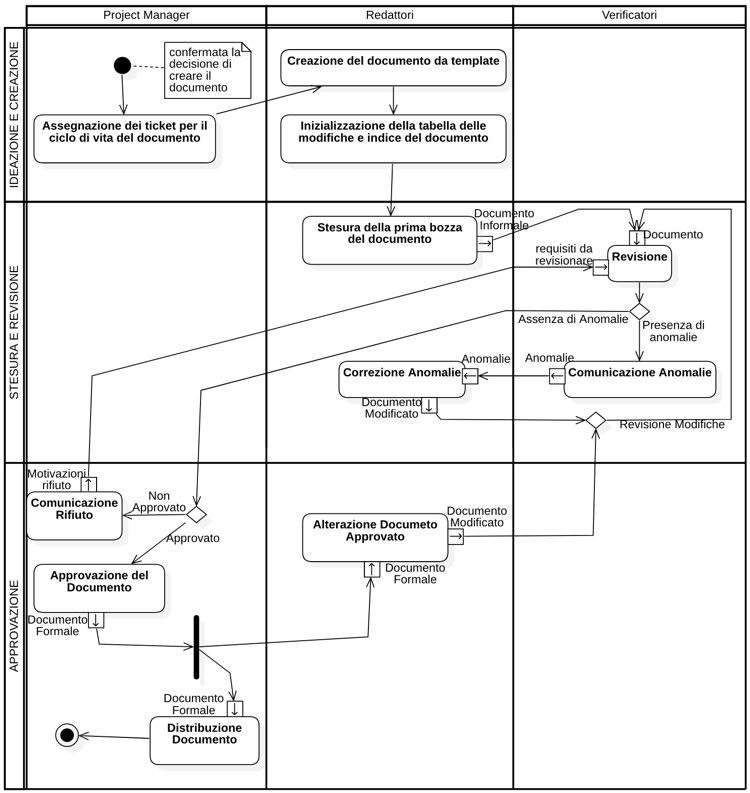
\includegraphics[width=1.0\textwidth]{res/images/ciclo_di_vita.png}
				\caption{Img.2 ciclo di vita della documentazione}
				\label{fig:Img.2 ciclo di vita della documentazione}
			\end{figure}
			\paragraph{Dal concepimento all’approvazione }
				I principali stadi del percorso che porta un documento formale dal suo concepimento alla sua approvazione sono:
				\begin{itemize}
					\item\textbf{Ideazione}:  La decisione di redigere lo specifico documento è stata confermata dal gruppo, vengono assegnati i ticket necessari per le varie fasi del suo ciclo di vita ai ruoli interessati;
					\item\textbf{Creazione}: il documento viene creato partendo da un template progettato per tale scopo situato nella cartella Template del repository remoto (vedi sezione §3.2.5.1). Alla prima creazione vengono inoltre inizializzati il registro delle modifiche e l’indice dei contenuti sulla base di tutte le informazioni disponibili in quel momento;
					\item\textbf{Stesura}: I membri del gruppo redigono il documento adottando un metodo incrementale: I membri devono essere predisposti ad accettare e risolvere a passi incrementali le correzioni proposte da coloro che effettuano la revisione.
					\item\textbf{Revisione}ogni sezione del corpo del documento viene regolarmente rivista da almeno un membro del gruppo, che deve essere obbligatoriamente diverso dal redattore della parte in verifica;
					\item\textbf{Approvazione}: terminata la revisione, il Responsabile del Progetto stabilisce la validità del documento, che solo a questo punto può essere considerato completo e può essere rilasciato.
				\end{itemize}
			\paragraph{Avanzamento di versione}
				Ogni volta che si effettueranno delle modifiche nel documento, queste verranno registrate in un apposito registro e classificate con un specifico codice. Questo varrà anche per il passaggio del documento da essere informale a diventare formale e definitivo.
				Per maggiori dettagli vedi sezione 3.3.2.1.


		\subsubsection{Struttura Documenti}
			\paragraph{Template utilizzati }
				Il gruppo ha deciso di adottare il linguaggio LATEX per la stesura dei documenti. \\
				Ogni documento dovrà essere realizzato a partire da un template LATEX appropriato reperibile al percorso 000, la scelta del template da utilizzare si basa sulla classificazione dei tipi di documenti esposta alla sezione 000.\\
				I template e gli script associati vanno utilizzati con lo scopo di semplificare, uniformare e automatizzare il più possibile la procedura di adeguamento alle norme per la redazione del documento.\\
			\paragraph{Struttura documento generico}
				\subparagraph{Frontespizio}
					Il frontespizio è la prima pagina di ogni documento formale e contiene: \\
					\begin{itemize}
						\item\textbf{Logo del progetto}
						\item\textbf{Nome del documento e data di ultima modifica}
						\item\textbf{Email identificativa del gruppo}: \href{mailto:everbuilds12@gmail.com}{everbuilds12@gmail.com}
						\item\textbf{Informazioni sul documento}, che includono: \\
							\begin{itemize}
								\item\textbf{Versione}: indica la versione corrente, approvata dal Responsabile del Progetto;
								\item\textbf{Uso}: indica la tipologia di uso che interessa il documento può essere:
									\begin{itemize}
										\item Interno
										\item Esterno
									\end{itemize}
								\item\textbf{Stato}: indica lo stadio corrente del ciclo di vita del documento può essere: 
									\begin{itemize}
										\item Creato
										\item In redazione
										\item In revisione
										\item Da approvare
										\item Approvato
									\end{itemize}
								\item\textbf{Redattori}: indica i membri di EverBuilds che si sono occupati della stesura del documento;
								\item\textbf{Verificatori}: indica i membri di EverBuilds che si sono occupati della verifica del documento;
								\item\textbf{Approvazione}: indica il nome dell’ultimo Responsabile di Progetto che ha approvato il documento.
							\end{itemize}
						\item\textbf{Sommario}: (opzionale) posto in fondo alla pagina, contiene una breve descrizione del contenuto del documento.
					\end{itemize}
				\subparagraph{Registro delle modifiche}
					Ogni documento presenta un registro delle modifiche, sotto forma di tabella, che tiene traccia di tutte le modifiche significative apportate al documento durante le fasi del suo ciclo di vita. \\
					Ogni riga del diario dovrà contenere i seguenti elementi: \\
					\begin{itemize}
						\item\textbf{Versione}: l numero di versione assegnato al documento. Tale numero viene assegnato in base alle norme previste nella sottosezione 000 relativa al versionamento;
						\item\textbf{Descrizione}: Campo composto dal codice numerico della sezione modificata e da una breve descrizione delle modifiche apportate;
						\item\textbf{Data}: Identifica la data in cui è avvenuta la modifica;
						\item\textbf{Autore}: Il soggetto che ha apportato le modifiche interessate dalla specifica riga;
						\item\textbf{Ruolo} : Il ruolo l’autore che ha assunto nell’eseguire la modifica.
					\end{itemize}
				\subparagraph{Indici}
					L’indice ha lo scopo di riepilogare e dare una visione macroscopica della struttura del documento, mostrando le parti gerarchiche di cui è composto. \\
					Saranno eventualmente presenti un indice delle figure e un indice delle tabelle, assenti in caso non ci siano tabelle o figure nel documento.
				\subparagraph{Corpo documento generico}
					Ogni pagina nel corpo del documento deve contenere i seguenti elementi:\\
					\begin{itemize}
						\item\textbf{Header}
							\begin{itemize} 
								\item In alto a sinistra si trova una miniatura a colori del logo del gruppo;
								\item In alto a destra si trova il nome del capitolo trattato nella pagina in considerazione.
							\end{itemize}
						\item\textbf{Contenuto} \\
							Il contenuto deve rispettare rigidamente le norme tipografiche espresse nel paragrafo 000 e garantite in parte dalla compilazione del template LATEX.
						\item\textbf{Note a piè pagina} \\
							In caso di presenza di note da esplicare, esse vanno indicate nella pagina corrente, in basso a sinistra. Ogni nota deve riportare un numero e una descrizione.
						\item\textbf{Footer}
							\begin{itemize} 
								\item In basso a sinistra, deve apparire il nome del documento e la sua ultima versione;
								\item In basso a destra, deve comparire il numero della pagina espresso in relazione al numero totale di pagine.
							\end{itemize}
					\end{itemize}
			\paragraph{Struttura documenti specializzati}
				\subparagraph{Struttura Verbale}
					Ai Verbali, sia interni che esterni, si applicano le medesime norme strutturali degli altri documenti esposte nella sezione 000. \\
					I Verbali aggiungono rispetto agli altri documenti i seguenti elementi strutturali:
					\begin{itemize}
						\item\textbf{Informazioni Generali}, composto dalle seguenti informazioni:
							\begin{itemize}
								\item Luogo: Dove si è tenuto l’incontro;
								\item Data: Data dell’incontro;
								\item Ora Inizio: Ora di inizio dell’incontro;
								\item Ora Fine: Ora di fine dell’incontro;
								\item Segretario: Il membro del gruppo che si è assunto il ruolo di segretario dell’incontro, cioè colui che ha il compito di redigere il documento.
								\item Partecipanti: Elenco delle persone presenti all’incontro.
							\end{itemize}
						\item\textbf{Resoconto}: descrizione degli argomenti trattati durante l’incontro, comprese le considerazioni che sono state fatte a riguardo;
						\item\textbf{Tabella delle Decisioni}: è una tabella che ci permette di tracciare le decisioni emerse dall’incontro. Lo scopo di tale tabella è quello di sfruttare al meglio il valore operativo del verbale. Il tracciamento è garantito dalla presenza di un codice univoco per ogni decisione che segue il seguente formalismo: \\
							\begin{center}
								\textbf{<Data verbale>\_<Numero decisione>}
							\end{center}
							Dove il numero di una decisione è assegnato in modo progressivo partendo da 1.
					\end{itemize}
				\subparagraph{Struttura Verbale}
					Al glossario si applicano le medesime norme strutturali degli altri documenti esposte alla sezione 000, oltre che alle seguenti ulteriori norme:\\
					\begin{itemize}
						\item I  termini sono ordinati secondo un criterio lessicografico; 
						\item Le lettere dell'alfabeto definiscono il primo e ultimo livello dell’albero gerarchico del documento e quindi dell’indice. Ogni capitolo sottende l’insieme dei termini che hanno come carattere iniziale la lettera che nomina il capitolo in questione; 
						\item I termini devono essere corredati da una descrizione concisa e che non sia fonte di ambiguità; 
						\item Un termine inizialmente può non contenere definizione. Tale modalità è da preferirsi al rimandare l’inserimento del termine nel glossario.
					\end{itemize}
				\subparagraph{Struttura Studio di Fattibilità}
					Allo Studio di Fattibilità si applicano le medesime norme strutturali degli altri documenti esposte alla sezione 000. \\
					I capitoli del corpo del documento espongono ciascuno uno dei capitolati proposti dal committente. I redattori, nell’esposizione di ciascun capitolato, devono compilare in modo esaustivo la lista di punti seguente: 
					\begin{itemize}
						\item\textbf{Informazioni Generali}, composto dalle seguenti informazioni:
							\begin{itemize}
								\item nome del capitolato;
								\item proponente
								\item committente
							\end{itemize}
						\item\textbf{descrizione del capitolato;}
						\item\textbf{finalità del progetto;}
						\item\textbf{tecnologie interessate;}
						\item\textbf{aspetti positivi;}
						\item\textbf{criticità e fattori di rischio;}
						\item\textbf{conclusioni.}
					\end{itemize}
					Per un maggiore dettaglio vedi sezione 000.
		\subsubsection{Norme tipografiche}
			\paragraph{Convenzioni di denominazione}
				I nomi dei file e delle directory, escludendo l’estensione del file utilizzano le seguenti convenzioni:\\
				\begin{itemize}
					\item i nomi composti da più parole usano il carattere underscore come carattere separatore;
					\item i nomi sono scritti interamente in minuscolo.
				\end{itemize}
				\subparagraph{Denominazione documenti formali}
					La denominazione dei documenti formali (a eccezione dei verbali) seguirà lo schema:  \\
					\begin{center}
						\textbf{<NomeDocumento>\_v<x>.<y>.<z>}
					\end{center}
					dove: \\
					\begin{itemize}
						\item\textbf{<NomeDocumento>}: corrisponde al nome ufficiale del documento; 
						\item\textbf{v} sta per versione e \textbf{<x>.<y>.<z>} rispettano quanto è indicato alla sezione §3.3.2.1 relativa al versionamento dei documenti
					\end{itemize}
				\subparagraph{Denominazione documenti informali}
					La denominazione dei documenti formali seguirà lo schema:  \\
					\begin{center}
						\textbf{<NomeDocumento>\_informale}
					\end{center}
					dove: \\
					\begin{itemize}
						\item\textbf{<NomeDocumento>}: corrisponde al nome ufficiale del documento.
					\end{itemize}
				\subparagraph{Denominazione Verbali}
					La denominazione dei Verbali seguirà lo schema:  \\
					\begin{center}
						\textbf{Verbale\_<tipo>\_<YYYY>-<MM>-<DD>}
					\end{center}
					dove: \\
					\begin{itemize}
						\item\textbf{<Tipo>}: corrisponde alla tipologia di Verbale e può assumere valori possibili pari a: interno / esterno;
						\item\textbf{<YYYY>-<MM>-<DD> }: corrisponde alla data in cui è avvenuto l’incontro.
					\end{itemize}
			\paragraph{Stili di testo e Punteggiatura}
				Gli stili adottati nei documenti sono: \\
				\begin{itemize}
					\item\textbf{Grassetto}: Per evidenziare il soggetto di una definizione, di un paragrafo o di un elemento di un elenco;
					\item\textbf{Corsivo}: Utilizzato per:
						\begin{itemize}
							\item Nomi propri, i nomi dei ruoli dei processi e delle attività;
							\item Nomi dei documenti, dei file e dei percorsi;
							\item Nomi delle tecnologie, degli strumenti, di formule matematiche, di termini specifici.
						\end{itemize}
					\item\textbf{Sottolineato}: Utilizzato quando il redattore vuole mettere in risalto il termine o frase perchè a suo giudizio è di rilevante importanza;
					\item\textbf{Glossario}: questo stile è caratterizzato dalla marcatura della parola in stile corsivo e da una ‘G’ corsiva a pedice, si applica esclusivamente per indicare che il termine ha una corrispondenza nel glossario. Se la voce viene ripetuta più volte nella stessa sezione, è sufficiente contrassegnata solo la prima volta che occorre;
					\item\textbf{Monospace}: tale stile viene adibito alla formattazione del testo contenente parti di codice o di comandi;
					\item\textbf{Maiuscolo}: l’utilizzo di parole le cui lettere sono tutte maiuscole dovrà limitarsi solo agli acronimi.
				\end{itemize}
				La punteggiatura adottata nei documenti rispetta le seguenti regole: \\
				\begin{itemize}
					\item\textbf{Punteggiatura}: deve essere utilizzata in modo attento per raggruppare parti di frase dal senso coeso e coerente. L’utilizzo del punto è richiesto per terminare un concetto e passare alla discussione di un altro argomento affine;
					\item\textbf{Spazi}: nessun segno di punteggiatura verrà anticipato da spazi, a meno delle parentesi aperte;
					\item\textbf{Parentesi tonde}: si utilizzano per sottendere una porzione di testo che se venisse rimossa il valore del paragrafo in cui si trova non verrebbe compromesso, esempi d’uso: per fornire un sinonimo del termine oppure un esempio;
					\item\textbf{Parentesi angolari}: Vengono utilizzate con funzione di escape per inserire all’interno di un esempio di formato dei segnaposti (e.g. formato png: \textbf{<NomeImmagine>.png}).
					\item\textbf{Virgolette}: le doppie virgolette si impiegano per indicare che l’insieme delle parole che sottendono hanno un’espressività più precisa e rigida rispetto semplicemente a ciò che significano, (e.g. “.. ma per seguir virtute e canoscenza” in questo caso è la sequenza esatta dei caratteri a conferire il significato ricercato);
					\item\textbf{Slash}: il simbolo ‘/’ si userà per indicare la disgiunzione esclusiva o la congiunzione tra due elementi testuali (e.g. inserire qui: testo/immagine ).
				\end{itemize}
			\paragraph{Composizione del testo}
				\begin{itemize}
					\item\textbf{Paragrafi}: i paragrafi devono essere sempre rientranti di 1 cm a sinistra dal margine della pagina e devono essere sempre giustificati;
					\item\textbf{Note a piè di pagine}: Nel caso in cui la nota a piè pagina dovesse essere ripetuta più volte di seguito, la si dovrà indicare un’unica volta e porre lo stesso indice per richiamare tale nota; 
					\item\textbf{Elenco}: Il simbolo per scandire un elenco puntato è il • (pallino); al livello successivo di annidamento, il simbolo usato è – (doppio trattino); al terzo livello è * (asterisco). Se si tratta di un elenco numerato, i tre livelli di enumerazione sono ordinati coi numeri arabi seguiti da un punto fermo (1.), con le lettere dell’alfabeto latino tra parentesi tonde ( (a) ) e dai numeri romani in caratteri minuscoli seguiti da punto fermo (i.) rispettivamente. Ogni voce di un elenco inizia con la lettera minuscola (tranne per i nomi propri), e termina con ; (punto e virgola), a meno che non si tratti dell’ultima voce, la quale termina con . (punto fermo). Le voci che corrispondono allo schema NomeElemento-descrizione presentano il primo termine della coppia in grassetto;
					\item\textbf{Esempi}: quando viene indicato un esempio, lo si deve fornire in linea con il testo, racchiuso tra parentesi tonde e usando il seguente formalismo
						\begin{center}
							\textbf{( e.g. <testo del esempio> )}
						\end{center}
				\end{itemize}
			\paragraph{Formati ricorrenti}
				\begin{itemize}
					\item\textbf{Date}: se non specificato in modo diverso, deve essere espressa seguendo il formalismo dello standard [ISO 8601]:\\
						\begin{center}
							\textbf{<AAAA>-<MM>-<GG>}
						\end{center}
						dove:\\
						\begin{itemize}
							\item\textbf{AAAA}: rappresenta l’anno. Per rappresentarlo si usano esattamente quattro cifre;
							\item\textbf{MM}: rappresenta il mese. Per rappresentarlo si usano esattamente due cifre;
							\item\textbf{GG}: rappresenta il giorno. Per rappresentarlo si usano esattamente due cifre.
						\end{itemize}
					\item\textbf{Orari}:  se non specificato in modo diverso, devono essere espressi seguendo il formalismo dello standard [ISO 8601]:\\
						\begin{center}
							\textbf{<HH>:<MM>}
						\end{center}
						dove:\\
						\begin{itemize}
							\item\textbf{HH}: rappresenta il numero di ore trascorse dalla mezzanotte, Per la rappresentazione vengono usate esattamente due cifre;
							\item\textbf{MM}: rappresenta i minuti. Per la rappresentazione vengono usate esattamente due cifre.
						\end{itemize}
					\item\textbf{Nomi ricorrenti}\\
						\begin{itemize}
							\item\textbf{Ruoli di progetto}: i ruoli di progetto andranno formattati con la prima lettera di ogni parola maiuscola a eccezione delle preposizioni e rappresentati in corsivo.
							\item\textbf{Nomi dei documenti e nomi di cartelle e file}: i vari nomi dei documenti andranno formattati con la prima lettera di ogni parola maiuscola a eccezione delle preposizioni, i nomi riportati di file e cartelle devono essere identici a i loro nomi effettivi case sensitive, i nomi di documenti file e cartelle sono rappresentati in corsivo e racchiusi tra doppie virgolette semplici. (e.g “Norme di Progetto”, “norme\_di\_progetto.tex”).
							\item\textbf{Riferimenti}per fare riferimento ad una sezione che fa parte dello stesso documento si deve scrivere il codice che la identifica preceduto dal simbolo: § (e.g §3.2). \\
								Per fare riferimento ad una sezione di un altro documento si riporta il nome del documento seguito da: § e il codice della sezione (e.g. “Norme di Progetto” §3.2).\\
						\end{itemize}
				\end{itemize}
			\paragraph{Sigle}
				si riportano le sigle fondamentali usate nei documenti per economicità di spazio
				\subparagraph{Sigle documenti}
					\begin{itemize}
						\item\textbf{AR} ad indicare il documento “Analisi dei Requisiti”;
						\item\textbf{PP} ad indicare il documento “Piano di Progetto”;
						\item\textbf{PQ} ad indicare il documento “Piano di Qualifica”;
						\item\textbf{NP} ad indicare il documento “Norme di Progetto”;
						\item\textbf{Gl} ad indicare il documento “Glossario”;
						\item\textbf{ST} ad indicare il documento “Specifica Tecnica”
					\end{itemize}
				\subparagraph{Processi}
					\begin{itemize}
						\item\textbf{FRN} ad indicare il processo di Fornitura.
						\item\textbf{SVL} ad indicare il processo di Sviluppo.
						\item\textbf{QLT} ad indicare il processo di Gestione della Qualità.
						\item\textbf{DCM} ad indicare il processo di Documentazione.
						\item\textbf{CNF} ad indicare il processo di Gestione della Configurazione.
						\item\textbf{PRB} ad indicare il processo di Gestione dei Problemi Accidentali.
						\item\textbf{VRF} ad indicare il processo di Verifica.
						\item\textbf{VLD} ad indicare il processo di Validazione.
						\item\textbf{CRD} ad indicare il processo di Coordinamento.
						\item\textbf{PNF} ad indicare il processo di Pianificazione.
					\end{itemize}
		\subsubsection{Stesura informale}
			In questa sezione sono descritti i suggerimenti che normano la stesura informale dei documenti per rendere questo procedimento efficace ed efficiente dalla parte dell’insieme dei redattori del documento.\\
			Con stesura informale dei documenti si intende quel procedimento svolto dai redattori per definire una bozza del documento utilizzando tecnologie come Google Docs.
			\paragraph{Evidenziazioni testuali}
				\begin{itemize}
					\definecolor{bubblegum}{rgb}{0.99, 0.76, 0.8}
					\item\colorbox{bubblegum}{Evidenziare un testo in rosa}: Serve a evidenziare un contenuto instabile difficilmente tracciabile che può subire una modifica a seguito di una decisione a monte, è utile in questo caso aiutarsi a tracciare con un commento questa dipendenza, (vedi sezione successiva).\\
				\end{itemize}
			\paragraph{Prefissi di commenti}
				Usare questi prefissi prima del testo del documento per uniformare l’intento del commento, velocizzare la ricerca dello stesso, (le parentesi quadre {[ ]} sono comprese nel prefisso)\\
				\begin{itemize}
					\item\textbf{[VEDI]}]: da usare quando il testo deve fare riferimento a una parte del repository o a sezioni di altri documenti o dello stesso documento ma il sistema ancora instabile e risulta imprudente stabilire in quel momento il riferimento definitivo; \\
					\item\textbf{[TODO]}: da usare quando la sezione è da completare ma è un compito che non è vincolato da conseguimenti esterni, come richieste di delucidazioni o decisioni all’intero gruppo; \\
					\item\textbf{[GRUPPO]}: indica una porzione di testo che richiede l’approvazione o l’intervento di uno o più membri esterni all’insieme di redattori dello specifico documento;
					\item\textbf{[PROGRESSIVO]}: indica che in quel punto deve essere aggiunto un numero progressivo riferito per esempio ad un’immagine, tabella o nota a piè pagina. \\
					\item\textbf{[PIÈ PAGINA]}: permette di definire un testo per la parola evidenziata che verrà inserito a piè pagina una volta formattato con LaTeX.
				\end{itemize}

		\subsubsection{Elementi grafici}
			\paragraph{Immagini}
				I formati delle immagini consentiti sono PDF e PNG. Tutte le immagini devono essere corredate da una breve didascalia che ne descriva il contenuto. Inoltre si deve fornire un numero progressivo ad ogni immagine nel documento per permetterne la tracciabilità. L’insieme di tutte le immagini presenti in un documento è riepilogato nella lista delle figure. \\
				La didascalia dell’immagine deve avere il seguente formato:
				\begin{center}
					\textbf{Img.<numero progressivo immagine> <Nome file immagine>: <Testo descrittivo>}
				\end{center}
				(e.g.  Img.3 vallata\_con\_albero.png: Una vallata con al centro un albero da frutto)
			\paragraph{Tabelle}
				Ogni tabella deve conformarsi rigidamente al template per la formattazione delle tabelle presente nel file: file 000. Ogni tabella deve essere corredata da una didascalia che ne esplicita lo scopo e il contenuto. Inoltre, deve essere provvista di numero progressivo. L’insieme di tutte le tabelle verrà indicato nella lista delle tabelle. \\
				La didascalia della tabella deve avere il seguente formato: \\
				\begin{center}
					\textbf{Tab.<numero progressivo tabella>: <Testo descrittivo>}
				\end{center}
				(e.g. Tab.5: la tabella mette in relazione i giorni della settimana con gli impegni dei componenti in ciascun giorno).
% rimosso per RR %
\iffalse
			\paragraph{Grafici UML}
				I grafici in linguaggio UML, usati per la modellazione dei casi d’uso e per i diagrammi della progettazione, sono inseriti come immagini.
\fi
		\subsubsection{Metriche}
			La presente sezione espone le metriche selezionate dal gruppo per misurare il raggiungimento degli obiettivi di qualità del processo di Documentazione. \\
			\paragraph{Comprensione}
				Per fornire una documentazione fruibile e comprensibile si è deciso di monitorare la sua qualità tramite delle metriche significative, ovvero le seguenti:\\
				\begin{itemize}
					\item\textbf{QM-PD-DOC01 Indice di Gulpease (GULP)}
						\begin{itemize}
							\item\textbf{Descrizione}: la metrica GULP permette di misurare la leggibilità di un documento basandosi sulla formula riportata di seguito;
							\item\textbf{Unità di misura}: numero intero
							\item\textbf{Formula}: \\
								\[GULP = 89+ \frac{300\times\#\mathit{frasi} -10\times\#lettere}{\#parole}\]
								
							\item\textbf{Risultato}: il risultato della formula ha i seguenti significati:
								\begin{itemize}
									\item se il risultato è pari 0 allora il documento non esiste e/o la sua leggibilità è terribile;
									\item se il risultato è maggiore di 40 allora il documento esiste ed è leggibile da chi possiede un diploma superiore;
									\item se il risultato è maggiore di 60 allora il documento esiste ed è leggibile da chi possiede una licenza media;
									\item se il risultato è maggiore di 80 allora il documento esiste ed è leggibile da chi possiede una licenza elementare;
									\item se il risultato è pari a 100 allora il documento esiste ed è molto più che leggibile.
								\end{itemize}
						\end{itemize}
					\item\textbf{QM-PD-DOC02 Correttezza ortografica(CORT)} 
						\begin{itemize}
							\item\textbf{Descrizione}: la metrica CORT permette di misurare la correttezza, a livello lessicografico, di un documento;
							\item\textbf{Unità di misura}: numero intero
							\item\textbf{Formula}: \\
								\[CORT = \# \mathit{numero\;di\;errori\;ortografici}\]
							\item\textbf{Risultato}: il risultato della formula ha i seguenti significati:
								\begin{itemize}
									\item se il risultato è pari 0 allora il documento non esiste o non ha errori ortografici;
									\item se il risultato è maggiore di 0 allora il documento esiste e presenta errori ortografici.
								\end{itemize}
						\end{itemize}
				\end{itemize}
		\subsubsection{Strumenti}
			\paragraph{LaTeX}
				Per la stesura dei documenti si è scelto di utilizzare il linguaggio di markup LaTeX. Il motivo principale che ha portato a questa scelta è la facilità di separazione tra contenuto e formattazione oltre che a consentire uno sviluppo orientato alla modularità, alla collaborazione e alla scalabilità.\\
				Come editor di testo il gruppo può scegliere di usare TEXstudio se si trova in un ambiente Windows oppure TEXShop se si trova in ambiente LINUX.  \\
			\paragraph{Google drive e Google Docs}
				Come citato al paragrafo 000, i redattori scelgono di adottare la tecnologia di scrittura di documenti testuali: Google Docs per redigere le prime bozze della documentazione a loro assegnata utilizzando il servizio web per la memorizzazione e sincronizzazione: Google Drive. \\
				La scelta si basa sulla facilità di utilizzo propria di questa tecnologia, su un sistema efficace per commentare il testo e sulla velocità di sincronizzazione del lavoro dei redattori che lavorano in parallelo, grazie all’utilizzo dell’ambiente di cloud computing: Google Drive. \\
			\paragraph{StarUML}
				Il software StarUML verrà adottato per la produzione di diagrammi di attività e diagrammi di casi d’uso necessarie per descrivere rispettivamente: parte delle attività riportate durante il processo Documentazione e i requisiti del prodotto analizzati nel documento “Analisi dei Requisiti”.
			\paragraph{Microsoft Excel}
				Utilizziamo il software della suite Microsoft Office per realizzare fogli elettronici. I fogli elettronici così creati ci serviranno per svolgere calcoli, produrre diagrammi, istogrammi e aerogrammi, creare tabelle e grafici.
			\paragraph{Google Sheet}
				Utilizziamo il software Google Sheet per realizzare i grafici necessari per rappresentare insiemi di dati a una o più dimensioni da inserire nella documentazione. La scelta si fonda anche sulla semplicità di fruibilità del software, data dall’accentramento di molteplici attività svolte all’interno dell’ambiente Google Drive.

	\subsection{Gestione della configurazione}
		\subsubsection{Introduzione processo}
			\paragraph{Descrizione}
				Il processo di gestione della configurazione raggruppa e organizza gli strumenti necessari alla produzione di documenti, codice e diagrammi, ma anche quelli necessari al versionamento e al coordinamento del gruppo.
			\paragraph{Obbiettivi}
				L’obiettivo della configurazione è gestire in modo ordinato e sistematico la produzione di documenti e codice. Un elemento soggetto a configurazione ha una collocazione, una denominazione e uno stato definiti. Per ogni oggetto configurato sono garantiti la modifica normata e il versionamento. \\
				Si vuole quindi unificare e uniformare lo stato degli strumenti usati durante lo svolgimento di tutto il progetto e classificare i prodotti dei vari processi implementati.
		\subsubsection{Versionamento}
			\paragraph{Codice di versione}
				Ogni documento deve avere una storia ricostruibile attraverso le sue versioni.  \\
				Ogni versione deve corrispondere a una riga della tabella delle modifiche. \\
				Il codice di versione è composto da 3 o più cifre: \\
				\begin{center}
					\textbf{<X>.<Y>.<Z>.<cifreAggiuntive>}
				\end{center}
				dove:
				\begin{itemize}
					\item\textbf{<X>} rappresenta la versione stabile del documento rilasciata al pubblico, approvata dal Responsabile di Progetto, che autorizza l’incremento del numero della versione. La numerazione inizia da 0;
					\item\textbf{<Y>} rappresenta una versione parzialmente stabile del documento, soggetta a verifica e approvazione da parte del Verificatore. Concettualmente potrebbe essere confrontato alla funzione dei test di integrazione nel software. La numerazione inizia da 0, viene incrementata dal Verificatore a ogni verifica, e riparte da questo valore ad ogni incremento di X;
					\item\textbf{<Z>} rappresenta una versione instabile del documento in quanto è in fase di elaborazione da parte dei redattori. Concettualmente potrebbe essere confrontato alla funzione dei test di unità nel software. La numerazione inizia da 0, viene incrementata dai redattori a ogni modifica, e riparte da questo valore ad ogni incremento di X o Y.
					\item\textbf{<cifreAggiuntive>} sono cifre separate da un punto ‘ . ‘ servono ad identificare delle sotto attività che sono state svolte per completare una fase di elaborazione da parte dei redattori/programmatori.
				\end{itemize}
			\paragraph{Scelta del sistema di versionamento}
				Per le parti del progetto da versionare si è scelto di usare il sistema di versionamento distribuito da Git, usando la repository di GitHub per ospitare la repository remota.
			\paragraph{Repository}
				Il gruppo EverBuilds ha deciso di spartire la mole di informazioni richiesta in più repository:
				\begin{itemize}
					\item una per il versionamento dei documenti redatti \url{https://github.com/everbuilds/Docs} ;
					\item per il versionamento del codice prodotto si farà affidamento su specifici repository git, al momento non specifichiamo il loro nominativo perché non sono stati ancora creati
				\end{itemize}
				Si è deciso di separare il codice dai documenti tenendo distinte le sezioni che riguardano la parte di implementazione da quelle che raccolgono la documentazione ad essa relativa.\\
			\paragraph{Struttura del repository}
				% Entrambi i tipi di repository sono organizzati in cartelle:
				\begin{itemize}
					\item\textbf{Documentazione}:
						\begin{itemize}
							\item\textbf{Template}: cartella contenente i file di template in linguaggio LATEX, usati per assemblare tutti i documenti. 
							\item\textbf{Esterni}: cartella contenente i documenti che saranno poi resi disponibili ai committenti e al proponente quali Analisi dei Requisiti, Piano di Progetto, Piano di Qualifica, Verbali esterni, Glossario, Lettera di presentazione;
							\item\textbf{Interni}: cartella contenente i documenti privati necessari al gruppo come Norme di Progetto, Studio di Fattibilità e Verbali interni.
							
						\end{itemize}
					% \item\textbf{Documentazione}: % altro da mettere più avanti
				\end{itemize}
				La suddivisione dei file per revisione favorisce una classificazione ordinata e una migliore tracciabilità dei prodotti della documentazione all’interno di ognuna di esse.
			\paragraph{Tipi di file}
				I file utilizzati per la documentazione del progetto sono:
				\begin{itemize}
					\item file con estensione ".tex" di LATEX;
					\item immagini con estensione ".png" o ".jpeg" da inserire nei documenti.
				\end{itemize}
				Il file .gitignore contiene un riferimento a tutti i file non versionati. Tale file è situato nel livello più esterno del repository.
			\paragraph{Comandi di GitHub}
				Il repository Docs è composto da diversi branch:
				\begin{itemize}
					\item\textbf{master}: su cui vengono riportati i documenti nella loro versione definitiva approvata dal Responsabile di Progetto e pronta per la consegna ai destinatari;
					\item\textbf{develop}: ramo di sviluppo in cui vengono riportati incrementalmente le modifiche apportate ai documenti e il codice, I documenti e il codice qui memorizzati devono essere stati verificati.
					\item\textbf{feature/<titoloIdentificativo>}: dove \textbf{<titoloIdentificativo>} è un titolo composto da parole con iniziali minuscole separate dal trattino ‘-’. Il titolo deve essere più descrittivo possibile per identificare il soggetto del branch cioè la feature da implementare.
				\end{itemize}
				Questa divisione è orientata ad uno sviluppo per feature, per cui, per lavorare alla stesura di un documento nel proprio repository locale, ogni membro del gruppo deve:
				\begin{enumerate}
					\item posizionarsi nel proprio repository locale;
					\item aprire un terminale;
					\item spostarsi sul ramo dedicato al documento cui deve lavorare, mediante il comando \texttt{git checkout} seguito dal nome del branch desiderato;
					\item eseguire il comando \texttt{git pull} per trasferire nel proprio repository locale eventuali modifiche apportate da altri membri del gruppo a quel ramo presenti in remoto;
					\item svolgere il lavoro assegnato, che può consiste nell'aggiunta di nuovo materiale o nella modifica di file già presenti;
					\item tornato sul terminale, eseguire il comando \texttt{git add} seguito dai nomi dei file che ha modificato;
					\item eseguire il comando \texttt{git commit -m} seguito da una breve descrizione del compito svolto;
					\item eseguire il comando \texttt{git push} per pubblicare il proprio lavoro sul repository remoto e renderlo visibile a tutti i membri del gruppo.
				\end{enumerate}
				
				\begin{figure}[H]
    					\centering
    					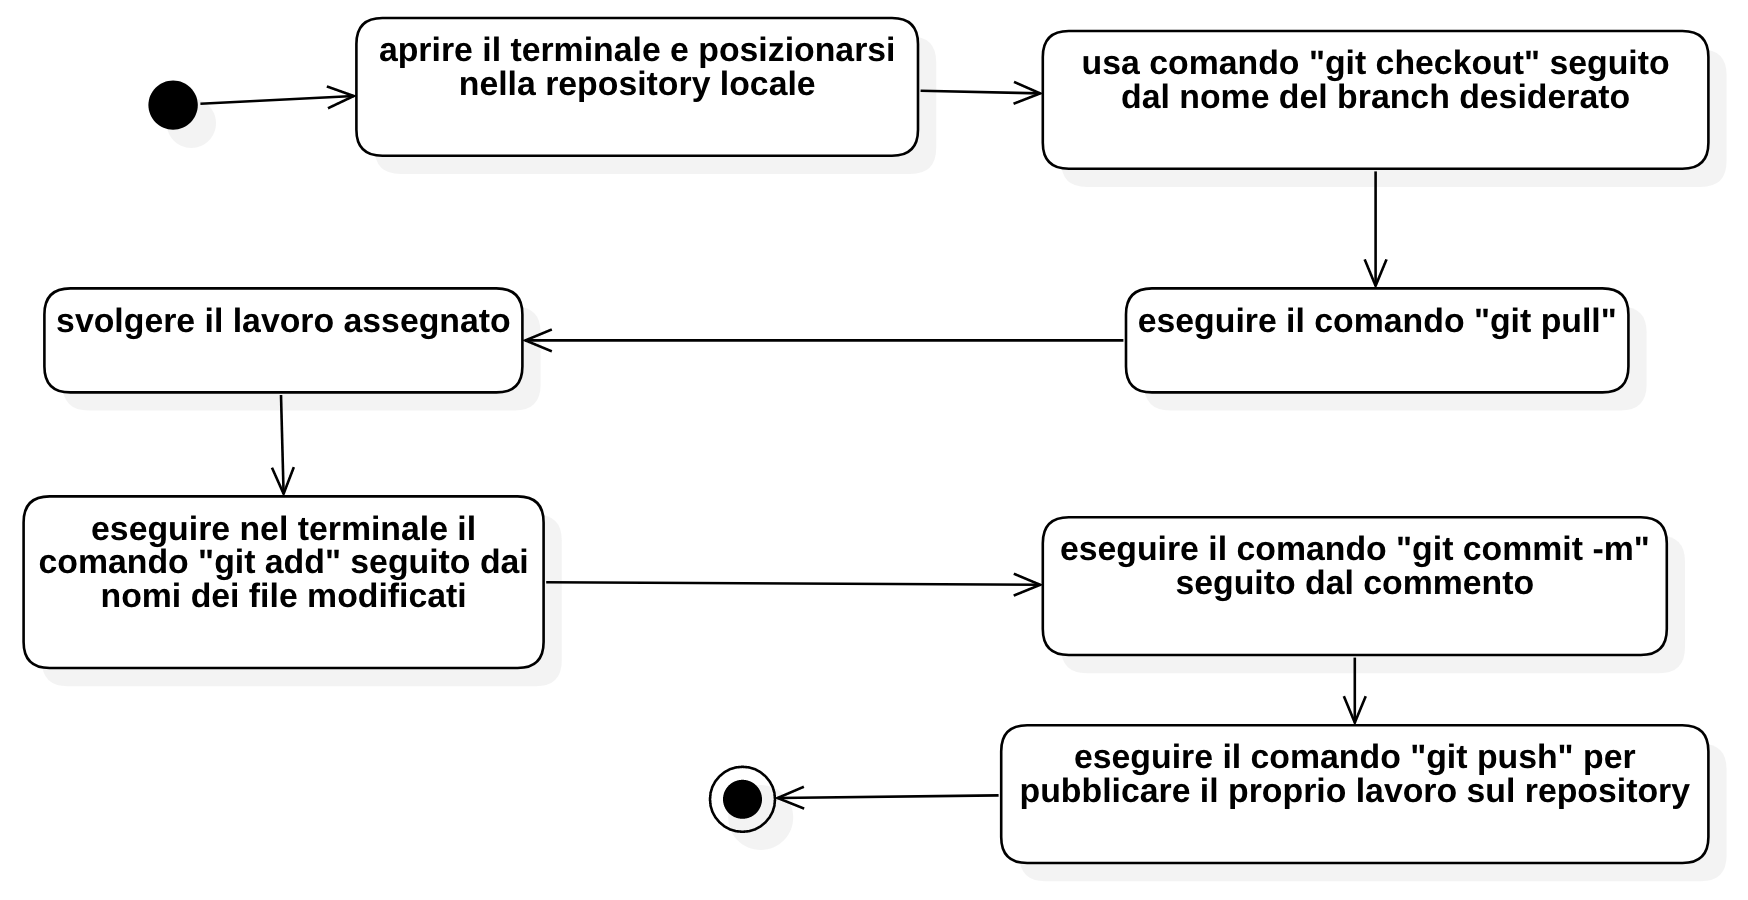
\includegraphics[width=1.0\textwidth]{res/images/comandi_GitHub.png}
					\caption{img.3 comandi_GitHub}
					\label{fig:img.3 comandi_GitHub}
				\end{figure}
				
				Un documento resta sul proprio ramo durante tutta la stesura e verifica.  \\
				Terminata la verifica, il documento viene spostato sul ramo \textbf{develop}, dove resterà fino a quando non sarà approvato dal Responsabile di Progetto. \\
				A quel punto, viene spostato sul ramo \textbf{master}.
				
			\paragraph{ Modifiche}
				Tutti i membri del team possono apportare modifiche ai file di ogni branch, ad eccezione dei file presenti nel ramo \textbf{master}, per i quali occorre fare una pull request ed ottenere l’approvazione di almeno un altro membro del gruppo. \\
				Per modifiche minime (sviste grammaticali, errori di battitura, problemi di lessico, questioni di impaginazione) è permessa la modifica autonoma da parte di qualunque membro del gruppo. \\
				Per modifiche maggiori sui contenuti o sulla struttura dei documenti già approvati è necessario contattare il Responsabile di Progetto che ha approvato il documento, esporgli le modifiche che si intendono effettuare con la relativa motivazione e nel caso sia valutata positivamente apportarla effettivamente al documento.\\
				In ambo i casi è opportuno commentare i propri commit con chiarezza per risalire facilmente alle modifiche.\\

	\subsection{Gestione dei problemi accidentali}
		\subsubsection{Introduzione Processo}
			\paragraph{Descrizione}
				Il processo di Gestione dei Problemi Accidentali definisce una procedura da seguire per analizzare e rimuovere dei problemi, qualsiasi sia la loro origine, scoperti durante l'esecuzione del processo di sviluppo, di manutenzione o di altri processi.
			\paragraph{Obbiettivi}
				L'obiettivo di questo processo è fornire un mezzo tempestivo, efficace ed per assicurarsi che tutti i problemi vengano analizzati, risolti, tracciati e, in un'ottica di miglioramento continuo, evitati.
			\paragraph{Aspettative}
			Il processo di “Gestione dei problemi accidentali” dovrà essere eseguito ogni volta che sarà necessario gestire un problema e dovrà soddisfare i seguenti requisiti: 
			\begin{itemize}
				\item tutti i problemi rilevati dovranno essere prontamente riportati ed immessi nel processo di gestione dei cambiamenti;
				\item dovranno essere avvisate prontamente le parti interessate;
				\item le cause dovranno essere identificate, analizzate e nel limite del possibile rimosse.
			\end{itemize}
		\subsubsection{Classificazione dei problemi accidentali}
			il processo deve assegnare un identificativo al problema categorizzarlo e dargli la giusta priorità, l’identificativo deve essere scritto nel seguente formato:
			\begin{center}
				\textbf{PRB:<priorità>-<numeroProgressivo>}
			\end{center}
			dove:
			\begin{itemize}
				\item\textbf{PRB}: sta per problema accidentale;
				\item\textbf{<priorità>}: indica il grado di urgenza con cui la risoluzione è richiesta, può assumere i seguenti valori:
					\begin{itemize}
						\item\textbf{A}: Priorità alta;
						\item\textbf{M}: Priorità media;
						\item\textbf{B}: Priorità bassa;
					\end{itemize}
				\item\textbf{<numeroProgressivo}: indica un numero progressivo all’interno dell’elenco di tutti i problemi accidentali.
			\end{itemize}
		\subsubsection{Issue di analisi del problema accidentale}
			Quando uno o più problemi saranno rilevati, nel prodotto software o in un'attività, dovrà essere interpellato il Responsabile del progetto il quale si propone di aprire una nuova issue di analisi del problema accidentale nell'ITS (Issue Tracking System) che conterrà:
			\begin{itemize}
				\item\textbf{Titolo}: il titolo corrisponde al codice identificativo del problema accidentale nel formato riportato alla sezione precedente;
				\item\textbf{Assegnatari}: Il responsabile aggiungerà il riferimento agli assegnatari della issue ovvero i verificatori che avranno il compito di aprire un processo di analisi della possibile criticità e nel limite del possibile sistemarla;
				\item\textbf{Commento}: Il commento conterrà le seguenti informazioni:
					\begin{itemize}
						\item Dove è stata riscontrata la problematica;
						\item Informazioni sullo stato del sistema in cui si è verificata la problematica;
						\item Come si può replicare la problematica.
					\end{itemize}				
			\end{itemize}	
		\subsubsection{Applicazione processo}
			Il processo di gestione di un problema accidentale dovrà seguire il flusso di lavoro rappresentato in questo diagramma:
			\begin{figure}[H]
    				\centering
    				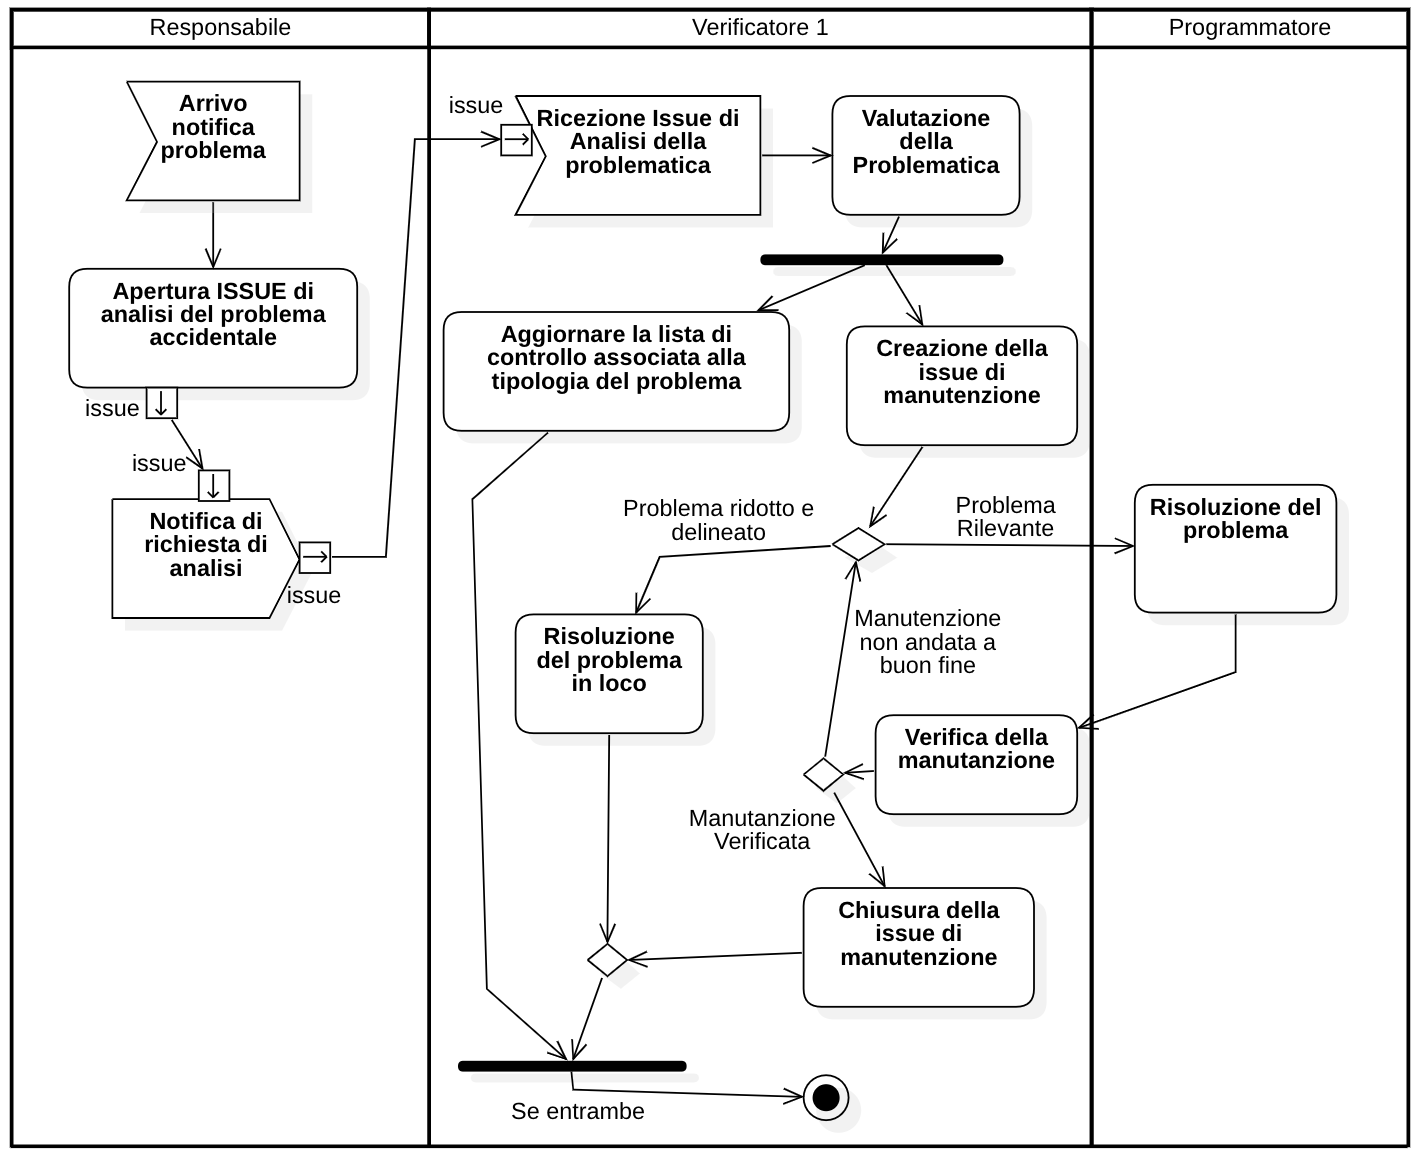
\includegraphics[width=1.0\textwidth]{res/images/gestione_problemi_accidentali.png}
				\caption{Img.4 gestione problemi accidentali}
				\label{fig:Img.4 gestione problemi accidentali}
			\end{figure}
		\subsubsection{Strumenti}
			\textbf{Github}: Questo ITS fornisce la possibilità di collegare la issue creata per analisi della problematica con la issue creata per la risoluzione della problematica.

	\subsection{Verifica}
		\subsubsection{Introduzione Processo}
			\paragraph{Descrizione}
				Il processo di Verifica prende in input un prodotto frutto di codifica (nel caso di un prodotto software) o di stesura (nel caso della documentazione), e ritorna in output la reportistica adeguata frutto di un’analisi che mira ad identificare le inadeguatezze del prodotto rispetto ai vincoli espressi nelle Norme di Progetto, e agli obiettivi di qualità espressi nel Piano di Qualifica. 
			\paragraph{Obbiettivi}
				Il processo consiste nella ricerca di anomalie e difetti nei processi e prodotti del progetto, mediante tecniche predefinite e se possibile automatiche. Sono soggetti a verifica il software e i documenti. Gli obiettivi della verifica sono:
				\begin{itemize}
					\item  individuare tecniche e strumenti di verifica;
					\item  individuare le anomalie applicando gli strumenti;
					\item  provare che il sistema soddisfi i requisiti.
				\end{itemize}
			\paragraph{Aspettative}
				Il corretto svolgimento del processo di verifica rispetta i punti seguenti:\\
				\begin{itemize}
					\item  Viene svolta seguendo procedure definite;
					\item  Deve definire criteri chiari e affidabili da seguire per verificare;
					\item  I prodotti transitano per diversi stadi ognuno dei quali deve essere verificato;
					\item  Permette di giungere all’attività di Validazione avendo garanzia che il prodotto abbia soddisfatto per tutto il suo ciclo di sviluppo i requisiti di realizzazione.
				\end{itemize}
				
		\subsubsection{Verifica Documentazione}
			Il processo di verifica attinente alla documentazione mette a disposizione dei verificatori due tecniche di indagine degli errori walkthrough e inspection, entrambe richiedono l’intervento manuale del verificatore. \\
			La procedure che descrivono lo svolgimento dell’attività di verifica sono rappresentate nel seguente diagramma delle attività \\
			\begin{figure}[H]
    				\centering
    				\includegraphics[width=1.0\textwidth]{res/images/attività_di_verifica.png}
				\caption{Img.5 attività di verifica}
				\label{fig:Img.5 attività di verifica}
			\end{figure}
			\paragraph{Walkthrough}
				Consiste in una lettura del testo cercando errori ed anomalie a largo spettro senza un’idea precisa di quali tipi errori sarà possibile trovare. Ogni difetto rilevato dai verificatori sarà discusso con i redattori del testo allo scopo di evitare incomprensioni e concordare sulle modifiche necessarie.\\
				Il walkthrough è indispensabile durante lo sviluppo iniziale, quando non si possiede ancora una chiara visione sui possibili errori. Usando più volte questa tecnica sarà possibile stilare una “lista di controllo” dove verranno archiviati gli errori più spesso rilevati. \\
				Inizialmente le attività di verifica utilizzano in prevalenza la tecnica walkthrough. Non appena i Verificatori avranno stilato una lista di controllo sufficiente, si passerà sempre più frequentemente all’uso della tecnica inspection.\\
			\paragraph{Inspection}
				L’inspection si basa sulla lettura mirata del testo. Durante tale lettura si cercano gli errori segnalati nelle liste di controllo appropriate, vedi sezione 000. Progressivamente con l’acquisizione di esperienza la lista di controllo verrà estesa. Questo renderà l’inspection sempre più efficace.

		\subsubsection{Verifica del codice}
			Il codice deve essere verificato dai verificatori adottando le strategie riportate in questa sezione, esse si basano su principi a cui devono tendere tutti i verificatori, progettisti e codificatori, questi criteri sono:
			\begin{itemize}
				\item  codice testabile, corretto e rispettoso di quando dichiarato dai requisiti e dallo standard di codifica adottato e dal way of working scelto dal gruppo
				\item il codice deve essere tracciato in un requisito a livello progettuale. 
				\item interfacce e dati consistenti e che minimizzano l’accoppiamento tra le componenti.
			\end{itemize}
			\paragraph{Analisi Statica}
				L’analisi statica non coinvolge unicamente la verifica dei documenti ma anche quella del codice prodotto. A fronte di questa osservazione si è scelto di impiegare per l’attività di analisi statica del codice le seguenti strategie
				\begin{itemize}
					\item\textbf{Walkthrough}: analogo alla strategia descritta alla sezione 000;
					\item\textbf{Inspection}: analogo alla strategia descritta alla sezione 000, con la differenza che le liste di controllo del codice adottate per svolgere l’attività si trovano alla sezione 000.
					\item\textbf{Analisi statica automatizzata}: Nel progetto utilizzeremo uno strumento per automatizzare l'analisi statica del codice, nel paragrafo successivo definiremo le regole che possono essere verificate in questo modo.
				\end{itemize}
				\subparagraph{Norme Analisi statica automatizzata}
					A tempo debito la sezione conterrà le norme e le configurazioni scelte per lo strumento di analisi statica del codice.
			\paragraph{Analisi Dinamica}
				L’analisi dinamica è una tecnica di verifica attuata testando il codice generato per mezzo della sua esecuzione. Su di esso vengono generati ed eseguiti una serie di test case, per verificarne il corretto funzionamento e per rilevare eventuali scostamenti tra i risultati ottenuti e quanto atteso. \\
				Tutti i test devono rispettare i seguenti criteri: \\
				\begin{itemize}
					\item Devono essere ripetibili
					\item Devono specificare l’ambiente di esecuzione e lo stato iniziale consentito
					\item Devono specificare gli input e output richiesti
					\item Devono notificare un eventuale esito negativo
					\item Devono fornire informazioni circa i risultati dell’ esecuzione.
					\item Se necessarie per una corretta comprensione del test devono riportare delle informazioni aggiuntive di tipo descrittivo.
				\end{itemize}
				\paragraph{Test unità}
					Test eseguiti sul funzionamento di unità di software in modo automatico: viene definito l'input e l'output atteso per verificare il corretto funzionamento dell'unità.\\
				\paragraph{Test di regressione}
					Test eseguito ogni volta che un'unità viene modificata allo scopo di trovare difetti nelle funzionalità già testate, potendo garantire che le funzionalità preesistenti non abbiano cambiato comportamento. Si ri-eseguono tutti i test necessari affinché si possa essere certi che la modifica non causi il funzionamento scorretto di altre unità collegate all'unità modificata.\\
				\paragraph{Test di integrazione}
					Test eseguiti su componenti del software per verificare se l'insieme di unità si interfaccia come dovrebbe. Questo test è eseguito in modo ricorrente: ogni volta che un insieme di unità esegue correttamente, esso viene integrato con altri insiemi di unità, fino al test completo sul sistema.\\
				\paragraph{Test di sistema}
					Dopo aver eseguito i test su tutte le unità e sulla loro integrazione, si testa il sistema nella sua interezza, si testa il comportamento delle componenti del sistema che devono risultare: compatibili tra di loro e sincronizzate nei comportamenti e coese nello spartirsi le responsabilità.\\
					I test di sistema caratterizzano la validazione del prodotto software finale, mezzo con il quale si verifica che tutti i requisiti siano soddisfatti in modo completo.\\
				\paragraph{Test di Accettazione}
					Anche detto test di collaudo È simile al test di sistema per l’oggetto testato, ma viene eseguito con la partecipazione dei committenti. Valida il prodotto e, in particolare, il soddisfacimento del cliente. Il superamento del test di collaudo garantisce che il software è pronto per essere rilasciato.
				\paragraph{Codice identificativo dei test}
					Per classificare le varie tipologie di test si utilizzerà il seguente formato:
					\begin{center}
						\textbf{<TipologiaTest>-<numeroProgressivo>}
					\end{center}
					dove:
					\begin{itemize}
						\item\textbf{<TipologiaTest> } è una sigla che itentifica uno dei 5 possibili tipi di test:
							\begin{itemize}
								\item\textbf{TU}: Test Unità;
								\item\textbf{TR}: Test di Regressione;
								\item\textbf{TI}: Test di Integrazione;
								\item\textbf{TS}: Test di Sistema;
								\item\textbf{TA}: Test di Accettazione.
							\end{itemize}
						\item\textbf{<numeroProgressivo>} identifica un numero progressivo all’interno della lista di una specifica tipologia di test.
					\end{itemize}
		\subsubsection{Metriche}
			Nella sezione verranno inserite a tempo debito le metriche selezionate dal gruppo per misurare il raggiungimento degli obiettivi di qualità del processo di Verifica.

	\subsection{Validazione}
		\subsubsection{Introduzione processo}
			\paragraph{Descrizione}
				Il processo di validazione prende in esame il prodotto in processo di verifica e fa sì che sia garantita la conformità ai requisiti espressi dal committente. Sarà compito del Responsabile di Progetto approvare il documento come validato.
			\paragraph{Obbiettivi}
				L’obiettivo è quello di stabilire se il prodotto soddisfa il compito per cui è stato creato. Dopo la validazione è garantito che il software rispetti i requisiti e che soddisfi i bisogni del committente.
		\subsubsection{Attività}
			Il processo di validazione deve identificare gli oggetti da validare, identificare una strategia con delle procedure di validazione in cui le procedure di verifica possono essere riutilizzate, applicare la strategia ed infine valutare che i risultati rispettino le aspettative.\\
			Sarà successivamente il Responsabile di Progetto che dovrà controllare i risultati ottenuti decidendo se accettare e approvare il documento oppure rigettare il documento, chiedendo un’ulteriore verifica del documento con nuove indicazioni o attuando una diversa strategia.\\
		\begin{center}
			\emph{Questa sezione verrà arricchita quando sarà necessario normare la validazione del codice.}
		\end{center}
\newpage
			
			
			
			
			